\selectlanguage{english}

\section{Schwarzschild black holes}

The simplest black hole solution is the Schwarzschild metric:
\begin{equation}
  ds^2 = - \left( 1 - \frac{2GM}{r} \right) dt^2 + \left( 1 - \frac{2GM}{r} \right)^{-1} dr^2 + r^2 \left( d\vartheta^2 + \sin^2 \vartheta\, d\varphi^2 \right)
  \label{eq:6.1}
\end{equation}
This is a special case of the general metric in Sec. \ref{ds-space} with $ f(r)^2 = 1 - 2GM / r $: it solves the vacuum Einstein equations $ R_{\mu \nu} = 0 $.\\
This solution depends on a single parameter $ M $, which is identified as the mass of the black hole: from the Newtonian approximation $ g_{00} = - (1 + 2\Phi) $, so $ \Phi = - \frac{GM}{r} $, which is precisely the potential for a point mass $ M $ at the origin. The same can be shown via Komar integrals: note that the Schwarzschild metric admits a timelike Killing vector field $ K = \pa_t $, with dual 1-form $ K = g_{00} dt $ and 2-form:
\begin{equation*}
  F = dK = - \frac{2GM}{r^2} dr \wedge dt
\end{equation*}
The associated Komar charge is:
\begin{equation*}
  M_{\text{Komar}} = - \frac{1}{8\pi G} \int_{\mathbb{S}^2_R} \star\, F = M
\end{equation*}
for all $ R > 2GM $ (radius of the horizon). Although the 2-form $ F $ obeys the vacuum Maxwell equations $ d\star F = 0 $, thus one would expect the associated Komar charge to vanish as there's no current, $ M_{\text{Komar}} = M \neq 0 $: this is possible because the mass of the black hole is localized at the origin, where $ F $ diverges. Moreover, the Schwarzschild solution is mathematically valid for $ M \in \R $: the solution $ M = 0 $ is just Minkowski spacetime, while $ M < 0 $ will be shown to be unphysical.

\subsection{Birkhoff theorem}

\begin{theorem}[Birkhoff]
  The Schwarzschild solution is the unique spherically-symmetric and asimptotically-flat solution to the vacuum Einstein field equations.
\end{theorem}
\begin{proof}
  First, spherical symmetry means that the metric has an $ \SOn{3} $ isometry. It can be shown that any metric with such isometry can be written as:
  \begin{equation*}
    ds^2 = g_{\tau \tau}(\tau, \rho) d\tau^2 + 2 g_{\tau \rho}(\tau, \rho) d\tau\,d\rho + g_{\rho \rho}(\tau, \rho) d\rho^2 + r^2(\tau, \rho) d\Omega_2^2
  \end{equation*}
  These coordinates make the $ \SOn{3} $ isometry manifest, as it acts on $ \mathcal{S}^2 $ leaving $ \tau $ and $ \rho $ unchanged: this is a \textit{foliation} of the space by $ \mathbb{S}^2 $. Being $ r(\tau,\rho) $ the size of the sphere, it is useful to change coordinates to $ \tau $ and $ r $:
  \begin{equation*}
    ds^2 = g_{\tau \tau}(\tau,r) d\tau^2 + 2g_{\tau r}(\tau,r) d\tau\,dr + g_{rr}(\tau,r) dr^2 + r^2 d\Omega_2^2
  \end{equation*}
  Note a subtlety: for some functions $ r(\tau,\rho) $ it's not possible to exchange $ r $ and $ \rho $ (ex.: $ r = \tau $), but these counterexamples are ruled out by the assumption that the spacetime is asymptotically the Minkowski spacetime. Now, to get rid of the cross-term, consider $ \tilde{t}(\tau,r) $:
  \begin{equation*}
    d\tilde{t}^2 = \left( \frac{\pa \tilde{t}}{\pa \tau} \right)^2 d\tau^2 + 2 \frac{\pa \tilde{t}}{\pa \tau} \frac{\pa \tilde{t}}{\pa r} d\tau\,dr + \left( \frac{\pa \tilde{t}}{\pa r} \right)^2 dr^2
  \end{equation*}
  It's always ppossible to pick $ \tilde{t}(\tau,r) $ such that the cross-term vanishes, so that:
  \begin{equation*}
    ds^2 = - f(\tilde{t},r) d\tilde{t}^2 + g(\tilde{t},r) dr^2 + r^2 d\Omega_2^2
  \end{equation*}
  Solving the Einstein field equations requires that $ f(\tilde{t},r) = h(\tilde{t}) f(r) $ and $ g(\tilde{t},r) = g(r) $, thus redefining $ h(\tilde{t}) d\tilde{t}^2 = dt^2 $ yields:
  \begin{equation*}
    ds^2 = - f(r) dt^2 + g(r) dr^2 + r^2 d\Omega_2^2
  \end{equation*}
  Note that, even though time-independence was not assumed, it was derived from the field equations: this metric has the timelike Killing vector $ K = \pa_t $, besides those from the $ \SOn{3} $ isometry. At this point, the field equations require that $ f(r) = g(r)^{-1} $, thus this metric reduces to that considered in Sec. \ref{geo-ds}: the Schwarzschild metric is the most general solution with $ \Lambda = 0 $.
\end{proof}

Therefore, the Schwarzschild metric does not only describe a black hole, but it describes the spacetime outside any non-rotating spherically-symmetric object, even in the presence of time-dependence (ex.: collapsing star).

\begin{definition}
  A spacetime is said to be \textit{stationary} if it admits a globally-timelike Killing vector field $ K $. In addition, being $ t $ the coordinate along the integral curves of $ K $, if it is invariant under $ t \rightarrow -t $, then it is said to be \textit{static}.
\end{definition}

The definition of static spacetime rules out $ dt dx $ cross-terms in the metric.

\begin{proposition}
  A spherically-symmetric metric must be static.
\end{proposition}
\begin{proof}
  By Birkhoff theorem.
\end{proof}

\subsection{Horizon}

The Schwarzschild metric diverges at $ r = 0 $ and $ r = 2GM \equiv R_s $. To distinguish between true singularities and coordinate singularities, the usual way is defining a coordinate-independent scalar quantity and studying it at divergence points.\\
Due to the vaccum field equations, the simplest scalars $ R $ and $ R_{\mu \nu} R^{\mu \nu} $ both vanish: the nect simplest curvature scalar is the \textit{Krentschmann scalar} $ R^{\mu \nu \rho \sigma} R_{\mu \nu \rho \sigma} $, which for the Schwarzschild metric is:
\begin{equation}
  R^{\mu \nu \rho \sigma} R_{\mu \nu \rho \sigma} = \frac{48 G^2 M^2}{r^6}
  \label{eq:6.2}
\end{equation}
At $ r = 2GM $, the Krentschmann scalar is $ \sim 1 / (GM)^4 $, suggesting that this is only a coordinate singularity: it turns out that's the case, and indeed the surface $ r = R_s $ is known as the \textit{event horizon} of the black hole. Note that, interestingly, heavier black holes have smaller curvature at the horizon.\\
On the contrary, $ r = 0 $ is a true singularity, simply known as the \textit{singularity} of the (classical) black hole.

\subsubsection{Near horizon limit}

To study the spacetime in the vicinity of the horizon, set $ r = 2GM + \eta $, with $ \eta \ll 2GM $. Moreover, consider $ \eta \in \R^+ $, thus restricting to the spacetime just outside the horizon. The metric then becomes at first order in $ \eta $:
\begin{equation*}
  ds^2 = - \frac{\eta}{2GM} dt^2 + \frac{2GM}{\eta} d\eta^2 + (2GM)^2 d\Omega_2^2
\end{equation*}
Spacetime is thus decomposed in a direct product of $ \mathbb{S}^2_{2GM} $ and a 2d Lorentzian manifold. Focusing on the latter, set $ \rho^2 = 8GM \eta $, so that:
\begin{equation*}
  ds^2 = - \left( \frac{\rho}{4GM} \right)^2 dt^2 + d\rho^2
\end{equation*}
This is called \textit{Rindler metric} and it is, in fact, just Minkowski spacetime:
\begin{equation*}
  T = \rho \sinh \left( \frac{t}{4GM} \right)
  \qquad
  X = \rho \cosh \left( \frac{t}{4GM} \right)
  \quad \Rightarrow \quad
  ds^2 = - dT^2 + dX^2
\end{equation*}
These are precisely the coordinates Eqq. \ref{eq:1.33}-\ref{eq:1.34} experienced by an observer undergoing constant acceleration $ a = 1 / (4GM) $: this makes sense, as an observer sitting at constant $ \rho $, i.e. constant $ r $, must accelerate in order not to fall into the black hole.\\
The outside of the black hole is $ (\rho,t) \in \R^+ \times \R $, corresponding to $ X > \abs{T} $. The horizon $ \rho = 0 $, instead, is mapped to the origin $ T = X = 0 $ of Minkowski space. However, note that the time coordinate is undefined at the origin since $ g_{00} = 0 $: scaling $ t \rightarrow \infty $ and $ \rho \rightarrow 0 $ keeping $ \rho e^{\pm t / 4GM} $ fixed makes it clear that the horizon actually corresponds to the lines:
\begin{equation*}
  r = 2GM \quad \Rightarrow \quad X = \pm T
\end{equation*}
Therefore, the event horizon is not a timelike surface (like the surface of a star), but a null surface.\\
Although the outside of the event horizon is only described by $ X > \abs{T} $, it is nonetheless possible to extend the metric to the whole Minkowski space $ X,T \in \R $: this makes it clear that the event horizon is not a real singularity, as nothing particular happens at $ X = \pm T $ (see Fig. \ref{rindler}). Zooming out, however, the peculiar properties of the horizon start to emerge from a global perspective.

\begin{figure}[b]
  \centering
  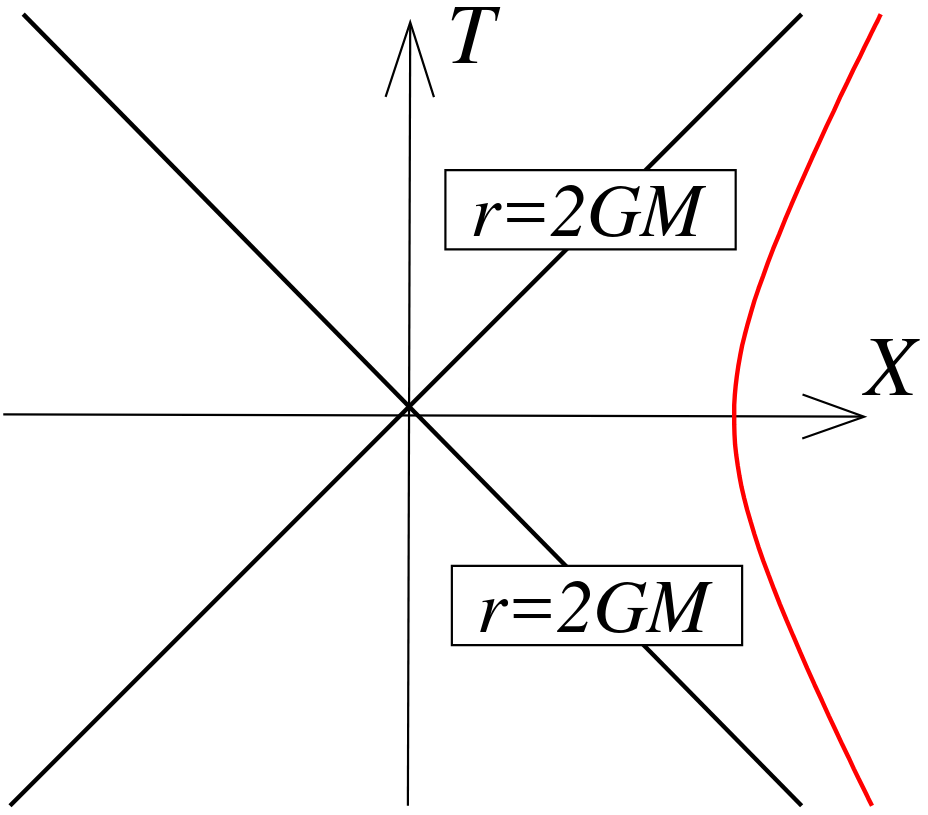
\includegraphics[width = 0.35 \textwidth]{rindler.png}
  \caption{Rindler spacetime, with null lines in black and a line at constant $ r > 2GM $ in red.}
  \label{rindler}
\end{figure}










